\documentclass{beamer}

\mode<presentation> {

%\usetheme{default}
%\usetheme{AnnArbor}
%\usetheme{Antibes}
%\usetheme{Bergen}
%\usetheme{Berkeley}
%\usetheme{Berlin}
%\usetheme{Boadilla}
%\usetheme{CambridgeUS}
%\usetheme{Copenhagen}
%\usetheme{Darmstadt}
%\usetheme{Dresden}
%\usetheme{Frankfurt}
%\usetheme{Goettingen}
%\usetheme{Hannover}
%\usetheme{Ilmenau}
%\usetheme{JuanLesPins}
%\usetheme{Luebeck}
\usetheme{Madrid}
%\usetheme{Malmoe}
%\usetheme{Marburg}
%\usetheme{Montpellier}
%\usetheme{PaloAlto}
%\usetheme{Pittsburgh}
%\usetheme{Rochester}
%\usetheme{Singapore}
%\usetheme{Szeged}
%\usetheme{Warsaw}


%\usecolortheme{albatross}
%\usecolortheme{beaver}
%\usecolortheme{beetle}
%\usecolortheme{crane}
%\usecolortheme{dolphin}
%\usecolortheme{dove}
%\usecolortheme{fly}
%\usecolortheme{lily}
%\usecolortheme{orchid}
%\usecolortheme{rose}
%\usecolortheme{seagull}
%\usecolortheme{seahorse}
%\usecolortheme{whale}
%\usecolortheme{wolverine}

%\setbeamertemplate{footline} % To remove the footer line in all slides uncomment this line
%\setbeamertemplate{footline}[page number] % To replace the footer line in all slides with a simple slide count uncomment this line

%\setbeamertemplate{navigation symbols}{} % To remove the navigation symbols from the bottom of all slides uncomment this line
}

\usepackage{graphicx} % Allows including images
\usepackage{booktabs} % Allows the use of \toprule, \midrule and \bottomrule in tables
\usepackage{amsfonts}
\usepackage{mathrsfs, bbold}
\usepackage{amsmath,amssymb,graphicx}
\usepackage{mathtools} % gather
\usepackage[export]{adjustbox} % right-aligned graphics

% argmax
\DeclareMathOperator*{\argmax}{arg\,max}

%----------------------------------------------------------------------------------------
%	TITLE PAGE
%----------------------------------------------------------------------------------------

\title["21"]{21: Gaussian Process Models}

\author{Taylor} 
\institute[UVA] 
{
University of Virginia \\
\medskip
\textit{} 
}
\date{} 

\begin{document}
%----------------------------------------------------------------------------------------

\begin{frame}
\titlepage 
\end{frame}

%----------------------------------------------------------------------------------------
\begin{frame}
\frametitle{Introduction}

We talk about Gaussian process models in this chapter. Gaussian processes describe random functions, and they can show up in statistical modeling in a few places. 
\newline

If you would like to dig a little deeper, this is considered a good reference: \url{http://gaussianprocess.org/gpml/}. The textbook's bibliography for this chapter includes many other sources.

\end{frame}
%----------------------------------------------------------------------------------------
\begin{frame}
\frametitle{Definitions}

It's helpful to initially consider $x_i \in \mathbb{R}^p$ where $p=1$ or $p=2$.
\newline

We say $\mu$ follows a {\bf Gaussian process} with mean function $m$ and covariance function $k$ if for any finite set of nonrandom points $x_1, \ldots, x_n$
$$
\mu(x_1), \ldots, \mu(x_n) \sim \text{Normal}( (m(x_1), \ldots, m(x_n)), K(x_1, \ldots, x_n)).
$$
For short, we write $\mu \sim \text{GP}(m,k)$. 
\pause
\newline

This means $E[\mu(x_i)] = m(x_i)$ and $\text{Cov}(\mu(x_i), \mu(x_j)) = K_{i,j} = k(x_i,x_j)$.
\newline


\end{frame}

%----------------------------------------------------------------------------------------
\begin{frame}
\frametitle{A first example: Gaussian process regression}

Let's assume we're regressing univariate $y_i$s on vector-valued $x_i$s. Then we are interested in 
$$
y_i = \mu(x_i) + \epsilon_i.
$$
We could also be interested in the ``noiseless" situation, as well. 
\newline

The $\mu$ function can be nonlinear and very flexible!

\end{frame}

%----------------------------------------------------------------------------------------
\begin{frame}
\frametitle{A first example: Gaussian process regression}

$$
y_i = \mu(x_i) + \epsilon_i.
$$

Picking a prior means we need to pick $m$ and $k$. We can see that 
$$
E[y_i \mid x_i] = E[\mu(x_i) \mid x_i] = m(x_i).
$$

For $m$
\begin{itemize}
\item can assume $m(x) = 0$ (like assuming regression coefficients have a zero-mean prior)
\item can use an informative prior
\end{itemize}

For $k$...

\end{frame}

%----------------------------------------------------------------------------------------
\begin{frame}
\frametitle{A popular choice}

Any $k$ function gives you a ``similarity" or ``nearness" measure for any two pairs of inputs. It needs to be chosen very carefully. 
\newline


We will often use a {\bf squared exponential kernel} 
$$
k(x,x') = \tau^2 \exp\left[-\sum_{i=1}^p \frac{ (x_j - x_j')^2 }{2 l_j^2} \right]
$$ 

Each $l_j$ determines the wiggliness in the $j$th direction of the predictors.
\newline

The $\tau^2$ parameter is an overall variance for each $\mu(x)$.
\newline


\end{frame}

%----------------------------------------------------------------------------------------
\begin{frame}
\frametitle{Simulating from the prior}


\begin{center}
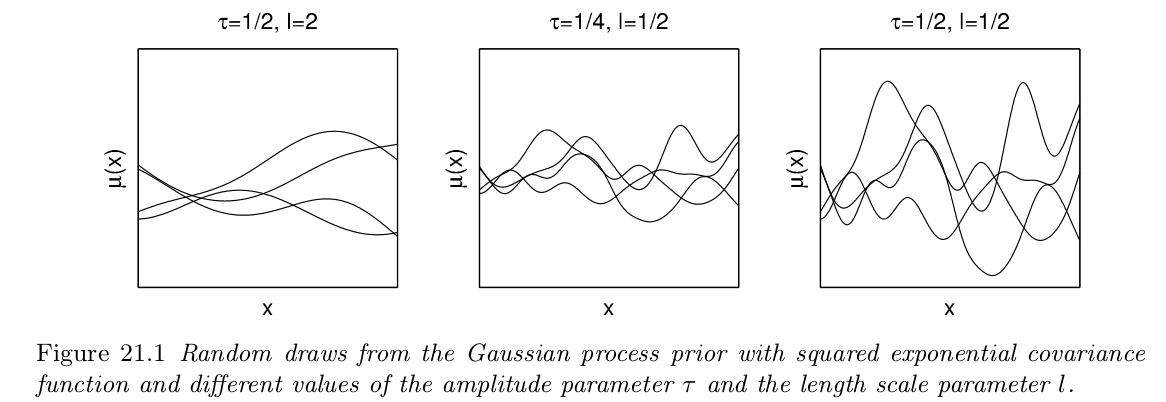
\includegraphics[width=120mm]{mu_realizations.png}
\end{center}

More to say about kernel choice: \url{https://www.cs.toronto.edu/~duvenaud/cookbook/}


\end{frame}
%----------------------------------------------------------------------------------------
\begin{frame}
\frametitle{Properties of Gaussian random vectors}

We will use a lot of properties of Gaussian random vectors when we conduct inference.
\newline

If 
$$
x = 
\left[\begin{array}{c}
x_1 \\
x_2
\end{array}\right]
\sim
\text{Normal}\left( 
\left[\begin{array}{c}
\mu_1 \\
\mu_2
\end{array}\right],
\left[\begin{array}{cc}
\Sigma_{11} & \Sigma_{12} \\
\Sigma_{21} & \Sigma_{22} 
\end{array}\right]
\right)
$$
then $x_1$ is also normally distributed with mean vector
$$
\mu_1 
$$
and covariance matrix
$$
\Sigma_{11} 
$$


\end{frame}

%----------------------------------------------------------------------------------------
\begin{frame}
\frametitle{Properties of Gaussian random vectors}

We will use a lot of properties of Gaussian random vectors when we conduct inference.
\newline

If 
$$
x = 
\left[\begin{array}{c}
x_1 \\
x_2
\end{array}\right]
\sim
\text{Normal}\left( 
\left[\begin{array}{c}
\mu_1 \\
\mu_2
\end{array}\right],
\left[\begin{array}{cc}
\Sigma_{11} & \Sigma_{12} \\
\Sigma_{21} & \Sigma_{22} 
\end{array}\right]
\right)
$$
then $x_1 \mid x_2$ is also normally distributed with mean vector
$$
\mu_1 + \Sigma_{12}\Sigma_{22}^{-1}(x_2 - \mu_2)
$$
and covariance matrix
$$
\Sigma_{11} - \Sigma_{12}\Sigma_{22}^{-1}\Sigma_{21}
$$


\end{frame}

%----------------------------------------------------------------------------------------
\begin{frame}
\frametitle{Inference: conditional posterior}


Let's assume the likelihood is $y_i = \mu(x_i) + \epsilon_i$ where $\epsilon_i \sim \text{Normal}(0,\sigma^2)$, and for the prior, $m(x) = 0$. 
\newline

The observed data is $\{x_i,y_i\}$, and the parameters are $\tau, l, \sigma^2$. To find the conditional posterior $p(\mu(x) \mid x,y,\sigma^2, \tau, l)$, we use
$$
\left(\begin{array}{c}
y \\
\mu
\end{array}\right) 
\bigg\rvert x, \sigma^2, \tau, l
\sim \text{Normal}\left(
\left(\begin{array}{c}
0\\
0
\end{array}\right),
\left(\begin{array}{cc}
K(x,x) + \sigma^2 I & K(x,x)\\
K(x,x) & K(x,x)
\end{array}\right)
\right)
$$
\pause

By properties of multivariate normal random vectors $\mu \mid x, y, \tau, l, \sigma$ is normally distributed with mean and covariance
\begin{align*}
E[\mu \mid x, y, \tau, l, \sigma] &= K(x, x) [K(x,x) + \sigma^2 I]^{-1} y \\
Var[\mu \mid x, y, \tau, l, \sigma] &= K(x, x) - K(x, x)[K(x,x) + \sigma^2 I]^{-1} K(x,x)
\end{align*}
\pause

What does this simplify to in the case of ``noiseless" regression?

\end{frame}

%----------------------------------------------------------------------------------------
\begin{frame}
\frametitle{Inference: conditional posterior}

\begin{center}
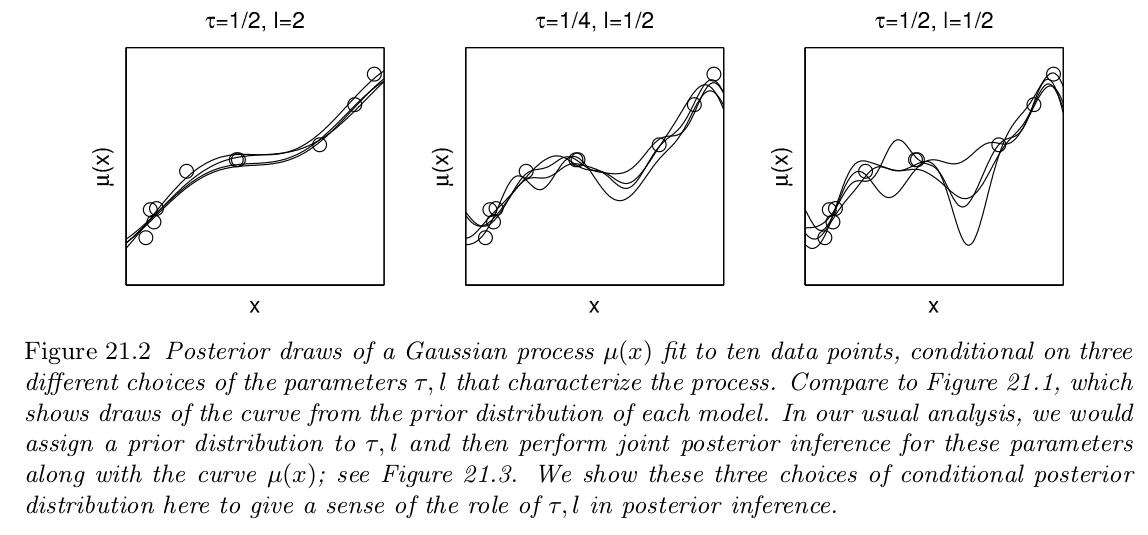
\includegraphics[width=120mm]{conditional_posterior.png}
\end{center}

\end{frame}
%----------------------------------------------------------------------------------------
\begin{frame}
\frametitle{Inference: prediction/smoothing at new points}


Let's assume the likelihood is $y_i = \mu(x_i) + \epsilon_i$ where $\epsilon_i \sim \text{Normal}(0,\sigma^2)$, and for the prior, $m(x) = 0$. 
\newline

Call $\tilde{x}$ unseen data, in addition to $\{x_i,y_i\}$. Then
$$
\left(\begin{array}{c}
y \\
\tilde{\mu}
\end{array}\right) 
\bigg\rvert x, \tilde{x}, \sigma^2, \tau, l
\sim \text{Normal}\left(
\left(\begin{array}{c}
0\\
0
\end{array}\right),
\left(\begin{array}{cc}
K(x,x) + \sigma^2 I & K(x,\tilde{x})\\
K(\tilde{x}, x) & K(\tilde{x}, \tilde{x})
\end{array}\right)
\right)
$$
By properties of multivariate normal random vectors, $\tilde{\mu} \mid x, y, \tau, l, \sigma$ is normally distributed with
\begin{align*}
E[\tilde{\mu} \mid x, y, \tau, l, \sigma] &= K(\tilde{x}, x) [K(x,x) + \sigma^2 I]^{-1} y \\
Var[\tilde{\mu}\mid x, y, \tau, l, \sigma] &= K(\tilde{x}, \tilde{x}) - K(\tilde{x}, x)[K(x,x) + \sigma^2 I]^{-1} K(x,\tilde{x})
\end{align*}

\end{frame}




%----------------------------------------------------------------------------------------
\begin{frame}
\frametitle{Inference: estimating unknown parameters}

We need the marginal likelihood for MCMC techniques: $\log p(y \mid \tau, l, \sigma^2)$ equals
$$
-\frac{n}{2}\log(2\pi) - \frac{1}{2}\log \det(K(x,x) + \sigma^2I) - \frac{1}{2} y^T [K(x,x) + \sigma^2I]^{-1} y
$$
We could use this to do Gibbs sampling or some sort of Metropolis-Hastings technique.
\newline

\end{frame}

%----------------------------------------------------------------------------------------
\begin{frame}
\frametitle{Birthdays and Birthdates example}

$$
y(t) = \mu(t) + \epsilon_t
$$
with
$$
\mu(t) = f_1(t) + f_2(t) + f_3(t) + f_4(t) + f_5(t).
$$

\end{frame}

%----------------------------------------------------------------------------------------
\begin{frame}
\frametitle{Birthdays and Birthdates example}

Slow and fast trends:

$$
f_1(t) \sim GP(0, k_1)
$$
$$
k_1(t,t') = \sigma_1^2 \exp\left[-\frac{(t-t')^2}{ 2l_1^2 } \right]
$$
and
$$
f_2(t) \sim GP(0, k_2)
$$
$$
k_2(t,t') = \sigma_2^2 \exp\left[-\frac{(t-t')^2}{ 2 l_2^2 } \right].
$$
There is an identifiability concern. They mention that they put log-t priors on $l_1$ and $l_2$ and log-uniform priors on $\sigma_1$ and $\sigma_2^2$, but they do not give specifics.

\end{frame}

%----------------------------------------------------------------------------------------
\begin{frame}
\frametitle{Birthdays and Birthdates example}

A quasi-periodic weekly effect:
$$
f_3(t) \sim GP(0, k_3)
$$
$$
k_3(t,t') = \sigma_3^2 \exp\left[-\frac{2\sin^2 (\pi[t-t']/7)}{ l_{3,1}^2 } \right]\exp\left[-\frac{(t-t')^2}{ 2 l_{3,2}^2 } \right].
$$
The kernel $k_3$ is ``high" only when both baby kernels are ``high."
\newline

Also note $2\sin^2 (\pi[t-t']/7) = 1 - \cos\left( \frac{2\pi [t-t']}{7} \right)$ by ``product identity."

\end{frame}
%----------------------------------------------------------------------------------------
\begin{frame}
\frametitle{Birthdays and Birthdates example}

A quasi-periodic yearly effect:
$$
f_4(t) \sim GP(0, k_4)
$$
$$
k_4(t,t') = \sigma_4^2 \exp\left[-\frac{2\sin^2 (\pi[t-t']/365.25)}{ l_{4,1}^2 } \right]\exp\left[-\frac{(t-t')^2}{ 2 l_{4,2}^2 } \right].
$$

\end{frame}

%----------------------------------------------------------------------------------------
\begin{frame}
\frametitle{Birthdays and Birthdates example}

Regular regression parameters

$$
f_5(t) = I_{\text{special day}}\beta_{a} + I_{\text{special day and weekend}}\beta_b
$$
where $I_{\text{special day}} = (I_{\text{New Year's Day} }, I_{\text{Valentine's Day} }, \ldots, I_{\text{Christmas} })'$.
\newline

$$
k_5(t,t') = ?
$$
\end{frame}



%----------------------------------------------------------------------------------------
\begin{frame}
\frametitle{Birthdays and Birthdates example}

This means 
$$
\mu(t) = f_1(t) + f_2(t) + f_3(t) + f_4(t) + f_5(t) \sim GP(0, k)
$$
where
$$
k(t,t') = k_1(t,t') + k_2(t,t') + k_3(t,t') + k_4(t,t') + k_5(t,t').
$$

\end{frame}



%----------------------------------------------------------------------------------------
\begin{frame}
\frametitle{Birthdays and Birthdates example}

\begin{center}
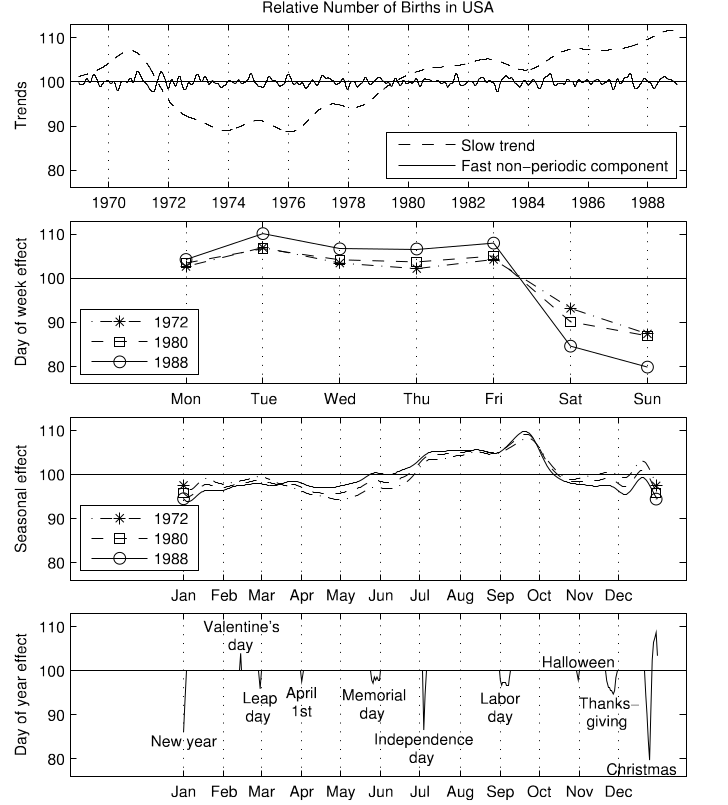
\includegraphics[width=70mm]{marginal_posterior.png}
\end{center}


\end{frame}



%----------------------------------------------------------------------------------------
\begin{frame}
\frametitle{The Catch}

All of this seems easy. We're just using normal-normal conjugacy, right?
\newline
\pause

Yes, but there are computational difficulties. For large data sets with more than several thousand rows, naively inverting $K(x,x) + \sigma^2I$ is going to be brutal.

\end{frame}

%----------------------------------------------------------------------------------------
\begin{frame}
\frametitle{Density estimation example}

So far we have discussed Gaussian processes as prior distributions for a function controlling
the location and potentially the shape parameter of a parametric observation model. 
\pause
\newline


To get more flexibility we would like to model also the conditional observation model as nonparametric.
\newline

One way to do this is with the {\bf logistic Gaussian proces} (LGP).
\end{frame}


%----------------------------------------------------------------------------------------
\begin{frame}
\frametitle{Density estimation example}

We want a density $p$ for random variables $y_1, \ldots, y_n \overset{\text{iid}}{\sim} p(y \mid f)$. 
\newline

So far this semester we have assumed $p$ is parametric (conditioning on parameters $\theta$). However, here, we want this density to be based on a nonparametric function $f$, which is a realization of a Gaussian process.
\newline
\pause

Recall that $p$ needs to be nonnegative, and it needs to integrate to $1$:
$$
p(y \mid f) = \frac{e^{f(y)} }{ \int e^{f(y)} \text{d}y }.
$$

\end{frame}
%----------------------------------------------------------------------------------------
\begin{frame}
\frametitle{Density estimation example}

Prior: $f \sim \text{GP}(m, k(\tau^2, l)) p(\tau^2, l)$
\newline

Likelihood: $\prod_{i=1}^n p(y_i \mid f)$. 

\end{frame}
%----------------------------------------------------------------------------------------
\begin{frame}
\frametitle{Density estimation example}

\begin{center}
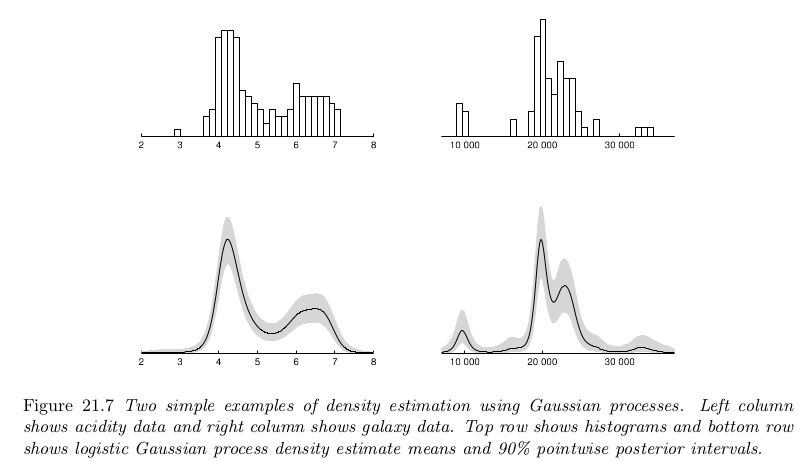
\includegraphics[width=90mm]{density_est.png}
\end{center}

\end{frame}

%----------------------------------------------------------------------------------------
\begin{frame}
\frametitle{Density estimation example}

$p$ is a density for random variables $y_1, \ldots, y_n \overset{\text{iid}}{\sim} p(y \mid f)$: 

$$
p(y \mid f) = \frac{e^{f(y)} }{ \int e^{f(y)} \text{d}y }.
$$

It is not possible to ``evaluate" the denominator because you cannot sample a mathematical function to be symbolically integrated. 
\newline

``In practice this integral is computed using a finite basis function representation or a discretization of a chosen finite region." 

\end{frame}




\end{document} 
